\documentclass{beamer}

\usepackage[T1]{fontenc}
\usepackage[utf8]{inputenc}

\usepackage{lmodern}

\usepackage{mathtools,amssymb}

\usepackage{graphicx}
\usepackage{xcolor}
\usepackage{tikz}

\usepackage{booktabs}
\usepackage{subcaption}

\usepackage{appendixnumberbeamer}

\definecolor{red_UCM}{HTML}{b01131}
\usetheme{Berlin}
\useoutertheme{infolines}
\useinnertheme{rectangles}
\usecolortheme[named=red_UCM]{structure}
\setbeamercolor{alerted text}{fg=red_UCM}

\usetikzlibrary{calc, positioning}
\AtBeginSection[]{\begin{frame}\tableofcontents[currentsection]\end{frame}}
% \setbeameroption{show notes}
\setbeamertemplate{note page}{\insertnote}
\addtobeamertemplate{note page}{}{\thispdfpagelabel{notes:\insertframenumber}}
\setbeamertemplate{navigation symbols}{}
\usebackgroundtemplate{\tikz[overlay,remember picture]\node[opacity=0.03125]at (current page.center){\includegraphics[scale=0.5]{images/UCM-logo.png}};}
\renewcommand\appendixname{Appendix}

\title[Jornadas de doctorandos]{Evolving Safely: Adaptation and Phenotypic Diversity under Environmental and Demographic Constraints}
\author[]
{
  \texorpdfstring{{\large Mendívil Carboni, Marco\inst{1}}\\\vspace{1ex} Dinis Vizcaíno, Luis Ignacio\inst{1} (dir.) \and Mazo Torres, Juan José\inst{1} (dir.)}{Marco Mendívil Carboni}
} 
\institute[Universidad Complutense de Madrid]
{
  \inst{1}
  Grupo Interdisciplinar de Sistemas Complejos (GISC) and Departamento de Estructura de la Materia, Física Térmica y Electrónica, Universidad Complutense de Madrid
}

\begin{document}

\frame{\titlepage}

\begin{frame}
  \tableofcontents
\end{frame}

\section{Introduction and objectives}

\begin{frame}
  \begin{columns}
    \hfill
    \begin{column}{0.6\textwidth}
      \begin{block}{Motivation}
        \begin{itemize}
          \item \alert{Adaptation} in fluctuating \alert{environments} is not fully understood yet.
          \item Especially under \alert{population limitations}.
          \item Paradigmatic example of \alert{fluctuations in biological processes}.
        \end{itemize}
      \end{block}
    \end{column}
    \begin{column}{0.4\textwidth}
      \begin{figure}
        \frame{\includegraphics[scale=0.08]{images/changing-environment.png}}
      \end{figure}
    \end{column}
  \end{columns}

  \begin{block}{Objectives}
    \begin{itemize}
      \item Develop a minimal mathematical \alert{model} to study this problem.
      \item Model the emergence of \alert{bet-hedging} strategies in fluctuating environments.
      \item Quantify how the \alert{evolutionary outcome} depends on these constraints.
      \item Identify the main mechanisms shaping these results and seek ways to \alert{approximate} them.
    \end{itemize}
  \end{block}

  \note[item]{Adaptation in fluctuating environments is a \alert{central problem} in \alert{evolutionary biology}.}
  \note[item]{Natural populations experience fluctuating rather than constant environments.}
  \note[item]{We will use a minimal mathematical model, \alert{not a detailed biological one}.}
  \note[item]{To investigate this, we will use \alert{numerical simulations}.}
  \note[item]{The main objective is to understand \alert{how populations adapt in fluctuating environments under demographic constraints}.}
  \note[item]{We wish to understand as well to what extent the strategies that emerge correspond to those of maximal growth or to safer, more resilient alternatives.}
\end{frame}

\section{The model: a Markov process}

\begin{frame}
  \begin{block}{System state}
    \begin{itemize}
      \item \alert{Environment}: $e\in\{1,2\}$, transition rates \alert{$\omega_t(e,e')$}
      \item \alert{Population}: $N$ agents, each one characterized by:
            \begin{itemize}
              \item \alert{phenotype}: $\phi\in\{A,B\}$
              \item \alert{strategy}: $s(\phi)$ (probability distribution)
            \end{itemize}
    \end{itemize}
  \end{block}
  \vfill
  \begin{figure}
    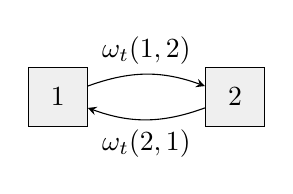
\begin{tikzpicture}[environment/.style={draw, minimum size=0.75cm, fill=lightgray!25}, >=stealth, node distance=2.25cm]
      \node[environment] (e1) {$1$};
      \node[environment, right of=e1] (e2) {$2$};
      \draw[->, bend left=20] (e1) to node[above] {$\omega_t(1,2)$} (e2);
      \draw[->, bend left=20] (e2) to node[below] {$\omega_t(2,1)$} (e1);
    \end{tikzpicture}
  \end{figure}

  \note[item]{\alert{Continuous-time} Markov process describing a population evolving in a fluctuating environment, that we will solve numerically using the \alert{Gillespie algorithm}.}
  \note[item]{The population starts with an initial number of agents \alert{$N_{\text{ini}}$}.}
  \note[item]{The environment is a \alert{discrete variable} that changes according to some transition rates.}
  \note[item]{The phenotype takes \alert{discrete values} as well.}
\end{frame}

\begin{frame}
  \begin{block}{Population Dynamics}
    \begin{itemize}
      \item \alert{Birth-Death}: environment- and phenotype-dependent birth and death rates \alert{$\omega_b(e,\phi)$} and \alert{$\omega_d(e,\phi)$}
      \item \alert{Evolution}: offsprings inherit the parent's strategy, mutations occur with probability \alert{$p_{\text{mut}}$}
      \item \alert{Constraint}: population size \alert{capped at $N_{\text{ini}}$}
    \end{itemize}
  \end{block}
  \vfill
  \begin{figure}
    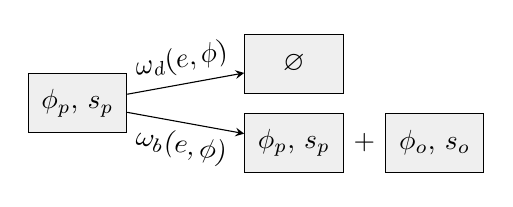
\begin{tikzpicture}[agent/.style={draw, minimum height=0.75cm, minimum width=1.25cm, fill=lightgray!25}, >=stealth, node distance=2.75cm]
      \node[agent] (parent) {$\phi_p$, $s_p$};
      \node[agent, right of=parent, yshift=+0.5cm] (death) {$\varnothing$};
      \node[agent, right of=parent, yshift=-0.5cm] (parent_copy) {$\phi_p$, $s_p$};
      \node[right=0cm of parent_copy, draw=none] (plus) {$+$};
      \node[agent, right=0cm of plus] (offspring) {$\phi_o$, $s_o$};
      \draw[->] (parent) -- node[sloped, midway, above] {$\omega_d(e,\phi)$} (death);
      \draw[->] (parent) -- node[sloped, midway, below] {$\omega_b(e,\phi)$} (parent_copy);
    \end{tikzpicture}
    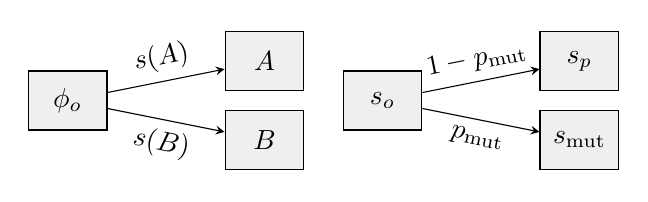
\begin{tikzpicture}[trait/.style={draw, minimum height=0.75cm, minimum width=1cm, fill=lightgray!25}, >=stealth, node distance=2.5cm]
      \node[trait] (phi_o) {$\phi_o$};
      \node[trait, right of=phi_o, yshift=+0.5cm] (A) {$A$};
      \node[trait, right of=phi_o, yshift=-0.5cm] (B) {$B$};
      \draw[->] (phi_o) -- node[sloped, midway, above] {$s(A)$} (A);
      \draw[->] (phi_o) -- node[sloped, midway, below] {$s(B)$} (B);
      \node[trait, right of=phi_o, xshift=1.5cm] (s_o) {$s_o$};
      \node[trait, right of=s_o, yshift=+0.5cm] (s_p) {$s_p$};
      \node[trait, right of=s_o, yshift=-0.5cm] (s_mut) {$s_{\text{mut}}$};
      \draw[->] (s_o) -- node[sloped, midway, above] {$1-p_{\text{mut}}$} (s_p);
      \draw[->] (s_o) -- node[sloped, midway, below] {$p_{\text{mut}}$} (s_mut);
    \end{tikzpicture}
  \end{figure}

  \note[item]{When an agent reproduces, the \alert{offspring's phenotype is drawn from the parent's strategy}.}
  \note[item]{\alert{Offspring inherit} the same \alert{phenotypic strategy} as their parent, allowing natural selection to act on strategies.}
  \note[item]{To allow \alert{evolution}, mutations are introduced: with a small probability at duplication, an agent's strategy \alert{mutates to a new random strategy}.}
  \note[item]{The total population size is \alert{capped at its initial value}, introducing a demographic constraint.}
\end{frame}

\begin{frame}
  \begin{block}{Parameters -- resistant vs. persistent}
    \begin{table}
      \begin{tabular}{c c c}
        \toprule
        symbol             & name                         & value                                                        \\
        \midrule
        $\omega_t(e,e')$   & environment transition rates & $\begin{psmallmatrix}-1.0&+1.0\\+1.0&-1.0\end{psmallmatrix}$ \\
        \addlinespace
        $\omega_b(e,\phi)$ & birth rates                  & $\begin{psmallmatrix}1.0&0.2\\0.0&0.0\end{psmallmatrix}$     \\
        \addlinespace
        $\omega_d(e,\phi)$ & death rates                  & $\begin{psmallmatrix}0.0&0.0\\1.0&0.1\end{psmallmatrix}$     \\
        \addlinespace
        $p_{\text{mut}}$   & mutation probability         & $0.001$                                                      \\
        \addlinespace
        $N_{\text{ini}}$   & initial number of agents     & $100$                                                        \\
        \bottomrule
      \end{tabular}
    \end{table}
  \end{block}

  \begin{block}{Types of simulations}
    \begin{enumerate}
      \item \alert{\texttt{fixed}}: \alert{common} initial strategy $s(\phi)_{\text{ini}}$, \alert{not evolving} ($p_{\text{mut}}=0$).
      \item \alert{\texttt{evol}}: \alert{common} initial strategy $s(\phi)_{\text{ini}}$, \alert{evolving}.
      \item \alert{\texttt{evol(r)}}: \alert{independent random} initial strategies, \alert{evolving}.
    \end{enumerate}
  \end{block}

  \note[item]{Environmental transition rates are equal and set to one, making \alert{both environments equally likely} for simplicity.}
  \note[item]{The environment alternates between a \alert{good} and a \alert{bad} state.}
  \note[item]{The \alert{resistant} phenotype grows fast in the good environment but dies quickly in the bad one, while the \alert{persistent} phenotype grows slowly but survives much better in bad conditions.}
  \note[item]{In \alert{fixed} simulations, all agents share the same strategy and \alert{evolution is suppressed}.}
  \note[item]{In \alert{evol} simulations, agents initially share a strategy, which evolves through \alert{mutation and selection}.}
  \note[item]{In \alert{evol(r)} simulations, agents start with independent random strategies, which then evolve.}
  \note[item]{Comparing the results of these three cases reveals the properties of the \alert{strategies} favored by selection, as we will see next.}
\end{frame}

\section{Results: phenotypic diversity and safe strategies}

\begin{frame}
  \begin{columns}
    \hfill
    \begin{column}{0.45\textwidth}
      \begin{block}{Observables}
        \begin{itemize}
          \item Average growth rate $\langle\mu\rangle=\left\langle\frac{1}{N(t)}\frac{dN}{dt}(t)\right\rangle$
          \item Total extinction rate $r_{\text{ext}}$
        \end{itemize}
      \end{block}
      \begin{block}{Take-home message}
        \alert{Growth-maximization} $\neq$ \alert{extinction-minimization}
      \end{block}
    \end{column}
    \begin{column}{0.55\textwidth}
      \begin{figure}
        \frame{\includegraphics[scale=0.75]{../sims/asymmetric/plots/strat_phe_0_i/avg_growth_rate.pdf}}
      \end{figure}
      \begin{figure}
        \frame{\includegraphics[scale=0.75]{../sims/asymmetric/plots/strat_phe_0_i/extinct_rate.pdf}}
      \end{figure}
    \end{column}
  \end{columns}

  \note[item]{These figures show the dependence of growth and extinction rates on the \alert{initial strategy} for different simulations.}
  \note[item]{Focusing on \alert{fixed} simulations we see that growth maximization and extinction minimization clearly \alert{do not coincide}.}
  \note[item]{Maximum growth occurs for strategies dominated (about \alert{80\%}) by the \alert{resistant} phenotype, while extinction is minimized by fully \alert{persistent} strategies.}
  \note[item]{This already indicates that we will have \alert{bet-hedging}.}
\end{frame}

\begin{frame}
  \begin{columns}
    \hfill
    \begin{column}{0.45\textwidth}
      \begin{block}{Observables}
        \begin{itemize}
          \item Average strategy $\langle s(A)\rangle$
          \item Distribution of strategies $p(s(A))$
        \end{itemize}
      \end{block}
      \begin{block}{Evolutionary outcome}
        \begin{itemize}
          \item Convergence to a \alert{common average strategy}.
          \item \alert{Independent} of initial conditions.
        \end{itemize}
      \end{block}
    \end{column}
    \begin{column}{0.55\textwidth}
      \begin{figure}
        \frame{\includegraphics[scale=0.75]{../sims/asymmetric/plots/strat_phe_0_i/avg_strat_phe_0.pdf}}
      \end{figure}
    \end{column}
  \end{columns}
  \vfill
  \begin{block}{Take-home message}
    Evolution selects a \alert{compromise} between growth-maximization and extinction-minimization.
  \end{block}

  \note[item]{We also compute the \alert{instantaneous standard deviation} of the strategy across agents.}
  \note[item]{Because strategies and the phenotype distribution are \alert{two-dimensional and normalized}, only one component is independent.}
  \note[item]{Both \alert{evol} and \alert{evol(r)} simulations converge to preety much the \alert{same average strategy}.}
  \note[item]{This indicates the presence of a \alert{stable attractor} in the space of strategies.}
  \note[item]{The \alert{strategy is common to almost all agents} at each instant, and thus talking about a \alert{common strategy} is meaningful.}
  \note[item]{This justifies comparing evolutive simulations with fixed-strategy simulations.}
  \note[item]{The \alert{selected strategy} lies \alert{between} the growth-maximizing and extinction-minimizing strategies.}
\end{frame}

\begin{frame}
  \begin{columns}
    \hfill
    \begin{column}{0.45\textwidth}
      \begin{block}{Population size dependence}
        \begin{itemize}
          \item Increasing \alert{$N_{\text{ini}}$} reduces \alert{extinction risk}.
          \item Evolution shifts toward the \alert{growth-maximizing strategy}.
          \item \alert{Small populations} favor \alert{safer strategies}.
        \end{itemize}
      \end{block}
      \begin{block}{Mutation probability dependence}
        \begin{itemize}
          \item \alert{Very weak} dependence.
          \item Mainly changes the \alert{effective lifetime} of strategies.
        \end{itemize}
      \end{block}
    \end{column}
    \begin{column}{0.55\textwidth}
      \begin{figure}
        \frame{\includegraphics[scale=0.75]{../sims/asymmetric/plots/n_agents_i/avg_strat_phe_0.pdf}}
      \end{figure}
      \begin{figure}
        \frame{\includegraphics[scale=0.75]{../sims/asymmetric/plots/prob_mut/avg_strat_phe_0.pdf}}
      \end{figure}
    \end{column}
  \end{columns}

  \note[item]{The evolutionary outcome depends on both the \alert{population size} and the \alert{mutation probability}.}
  \note[item]{As $N_{\text{ini}}$ increases, extinction becomes rare and the selected strategy approaches the \alert{growth-maximizing one}.}
  \note[item]{For \alert{small populations}, extinction risk is substantial, and evolution favors \alert{safer strategies} with lower extinction probability.}
  \note[item]{The mutation probability mainly controls the \alert{exploration of strategy space}.}
  \note[item]{The dependence on $p_{\text{mut}}$ is very weak, indicating a \alert{robust evolutionary attractor} that does not depend strongly on the mutation kernel. This is confirmed by simulations with \alert{incremental mutations}.}
\end{frame}

\begin{frame}
  \begin{columns}
    \hfill
    \begin{column}{0.45\textwidth}
      \begin{block}{Heuristic approximation}
        Stationary distribution of strategies:
        \begin{equation*}
          p(s)\propto\frac{\exp\left(N_\text{ini}\langle\mu(s)\rangle\right)}{r_{\text{ext}}(s)+p_{\text{mut}}\langle\mu_b\rangle}
        \end{equation*}
      \end{block}
      \begin{block}{Interpretation}
        \begin{itemize}
          \item \alert{Numerator}: expected exponential growth of a strategy during competition.
          \item \alert{Denominator}: loss of strategies through extinction and mutation fixation.
        \end{itemize}
      \end{block}
    \end{column}
    \begin{column}{0.55\textwidth}
      \begin{figure}
        \frame{\includegraphics[scale=0.66]{../sims/asymmetric/plots/fixed/exp_avg_strat_phe_0.pdf}}
        \caption*{\footnotesize Expected average strategy}
        \frame{\includegraphics[scale=0.66]{../sims/asymmetric/plots/fixed/avg_strat_phe_0.pdf}}
        \caption*{\footnotesize Measured average strategy}
      \end{figure}
    \end{column}
  \end{columns}

  \note[item]{To explain the evolutionary outcome we have come up with a \alert{heuristic approximation} for the stationary distribution of strategies.}
  \note[item]{The numerator represents the expected exponential expansion of a strategy.}
  \note[item]{When several strategies compete, this exponential growth determines the probability that a given strategy is selected.}
  \note[item]{The denominator represents the \alert{loss rate} of strategies due to extinction and mutation-driven replacement.}
  \note[item]{All quantities entering this expression are measured in \alert{fixed-strategy simulations}.}
\end{frame}

\section{Conclusions and future work}

\begin{frame}
  \begin{block}{Conclusions}
    \begin{itemize}
      \item Bet-hedging emerges \alert{naturally} in this minimal stochastic model.
      \item Populations evolve toward \alert{common or very similar strategies}.
      \item Evolution does \alert{not necessarily maximize growth}.
      \item Demographic constraints shift selection toward \alert{safer strategies}.
      \item We quantitatively understand the interplay between \alert{selection, extinction, and mutation}.
    \end{itemize}
  \end{block}

  \begin{columns}
    \hfill
    \begin{column}{0.5\textwidth}
      \begin{block}{Future work}
        \begin{itemize}
          \item Improve the heuristic stationary \alert{distribution of strategies}.
          \item Extend the model to environment-dependent strategies (\alert{sensing}).
        \end{itemize}
      \end{block}
    \end{column}
    \begin{column}{0.5\textwidth}
      \begin{figure}
        \frame{\includegraphics[scale=0.1]{images/sensing.png}}
      \end{figure}
    \end{column}
  \end{columns}

  \note[item]{The evolutionary outcome depends \alert{not only on average instantaneous} properties.}
  \note[item]{It is also shaped by the frequency of rare events such as \alert{extinction} and \alert{mutation fixation}.}
\end{frame}

\section*{Acknowledgments}

\begin{frame}
  \vfill
  \begin{center}
    \vfill
    \Large{Thank you for your attention.}
    \vfill
  \end{center}
  \vfill
  \begin{figure}
    \includegraphics[width=0.4\textwidth]{images/MICIU-logo.pdf}
  \end{figure}
\end{frame}

\appendix

\section*{Numerical methods}

\begin{frame}
  \begin{block}{Gillespie algorithm}
    \begin{equation*}
      \Omega(\mathbf{X})=\sum_{j=1}^M\omega_j(\mathbf{X})
    \end{equation*}
    \begin{equation*}
      \tau=\frac{1}{\Omega(\mathbf{X})}\ln\frac{1}{r_1},\ r_1\sim U(0,1)
    \end{equation*}
    \begin{equation*}
      \sum_{j=1}^{\mu-1}\omega_j(\mathbf{X})<r_2\Omega(\mathbf{X})\le\sum_{j=1}^{\mu}\omega_j(\mathbf{X}),\ r_2\sim U(0,1)
    \end{equation*}
    \begin{equation*}
      \mathbf{X}(t+\tau)=\mathbf{X}(t)+\boldsymbol{\nu}_\mu
    \end{equation*}
  \end{block}
\end{frame}

\section*{Symmetric parameters}

\begin{frame}
  \begin{columns}
    \begin{column}{0.5\textwidth}
      \begin{figure}
        \frame{\includegraphics[scale=0.75]{../sims/symmetric/plots/strat_phe_0_i/avg_growth_rate.pdf}}
      \end{figure}
      \begin{figure}
        \frame{\includegraphics[scale=0.75]{../sims/symmetric/plots/strat_phe_0_i/extinct_rate.pdf}}
      \end{figure}
    \end{column}
    \begin{column}{0.5\textwidth}
      \begin{figure}
        \frame{\includegraphics[scale=0.75]{../sims/symmetric/plots/strat_phe_0_i/avg_strat_phe_0.pdf}}
      \end{figure}
      \begin{figure}
        \frame{\includegraphics[scale=0.75]{../sims/symmetric/plots/n_agents_i/avg_strat_phe_0.pdf}}
      \end{figure}
    \end{column}
  \end{columns}
\end{frame}

\section*{Incremental mutations}

\begin{frame}
  \begin{figure}
    \frame{\includegraphics[scale=0.75]{../sims/incremental/plots/strat_phe_0_i/avg_strat_phe_0.pdf}}
  \end{figure}
  \begin{figure}
    \frame{\includegraphics[scale=0.75]{../sims/incremental/plots/n_agents_i/avg_strat_phe_0.pdf}}
  \end{figure}
\end{frame}

\end{document}
